\begin{enumerate}[\bfseries \textbf{Ejercicio} 1.]

    %-------------------- 1.
    \item \textbf{Demuestre vectorialmente la ley de los senos y cosenos.\\\\
	Demostración.-}\; Demostremos la ley de los senos. Considere el siguiente triangulo.
	\begin{center}
	    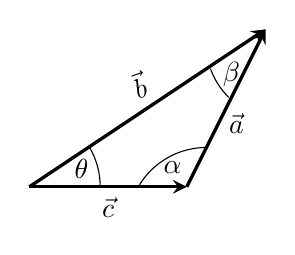
\begin{tikzpicture}[scale=1]
		\draw[line width=1.2pt,-stealth](0,0)--(2,0) node[rotate=0,pos=0.5, below]{$\vec{c}$};
		\draw[line width=1.2pt,-stealth](2,0)--(3,2) node[rotate=0,pos=0.4, right]{$\vec{a}$};
		\draw[line width=1.2pt,-stealth](0,0)--(3,2) node[rotate=20,pos=0.5, above]{$\vec{b}$};
		\draw(.9,0) arc (0:30:1)node[pos=.43,left]{$\theta$};
	        \draw(2.25,.5) arc (90:150:1)node[pos=.7,right]{$\alpha$};
	        \draw(2.3,1.5) arc (200:225:1)node[pos=.2,right]{$\beta$};
	    \end{tikzpicture}
	\end{center}
	Sea $\vec{a},\vec{b},\vec{c} \in V_3$. Notemos que $\vec{b}=\vec{c}+\vec{a}$ por lo que utilizaremos la proposición $$\|\vec{x} \times \vec{y}\| = \|\vec{x}\|\|\vec{y}\| \sen(\theta)$$
	de la siguiente manera. Sea $x\times x = 0$ de donde,
	\begin{itemize}

	    \item $\sen(\theta) = \dfrac{\|\vec{b}\times \vec{c}\|}{\|\vec{b}\|\|\vec{c}\|}=\dfrac{\|(\vec{c}+\vec{a})\times \vec{c}|\|}{\|\vec{b}\|\|\vec{c}\|}=\dfrac{\|\vec{c}\times \vec{c} + \vec{a}\times \vec{c}\|}{\|\vec{b}\|\|\vec{c}\|}=\dfrac{\|\vec{a}\times \vec{c}\|}{\|\vec{b}\|\|\vec{c}\|}.$ Entonces,
		$$\dfrac{\sen(\theta)}{\|\vec{a}\|}=\dfrac{\|\vec{a}\times \vec{c}\|}{\|\vec{a}\|\|\vec{b}\|\|\vec{c}\|}$$

	    \item $\sen(\alpha) = \dfrac{\|\vec{c}\times \vec{a}\|}{\|\vec{a}\|\|\vec{c}\|}=\dfrac{\|(\vec{b}-\vec{a})\times \vec{a}|\|}{\|\vec{a}\|\|\vec{c}\|}=\dfrac{\|\vec{a}\times \vec{b} - \vec{a}\times \vec{a}\|}{\|\vec{a}\|\|\vec{c}\|}=\dfrac{\|\vec{a}\times \vec{b}\|}{\|\vec{a}\|\|\vec{c}\|}.$ Entonces,
		$$\dfrac{\sen(\alpha)}{\|\vec{b}\|}=\dfrac{\|\vec{a}\times \vec{c}\|}{\|\vec{a}\|\|\vec{b}\|\|\vec{c}\|}$$

	    \item $\sen(\beta) = \dfrac{\|\vec{b}\times \vec{a}\|}{\|\vec{a}\|\|\vec{b}\|}=\dfrac{\|(\vec{c}+\vec{a})\times \vec{a}|\|}{\|\vec{a}\|\|\vec{b}\|}=\dfrac{\|\vec{c}\times \vec{a} - \vec{a}\times \vec{a}\|}{\|\vec{a}\|\|\vec{b}\|}=\dfrac{\|\vec{a}\times \vec{c}\|}{\|\vec{a}\|\|\vec{b}\|}.$ Entonces,
		$$\dfrac{\sen(\beta)}{\|\vec{c}\|}=\dfrac{\|\vec{a}\times \vec{c}\|}{\|\vec{a}\|\|\vec{b}\|\|\vec{c}\|}$$

	\end{itemize}
	Por lo tanto,
	$$\dfrac{\sen(\theta)}{\|\vec{a}\|}=\dfrac{\sen(\alpha)}{\|\vec{b}\|}=\dfrac{\sen(\beta)}{\|\vec{c}\|}.$$\\

	Ahora demostremos el teorema de los cosenos. La siguiente gráfica nos dará una idea de lo que se quiere demostrar.
	\begin{center}
	    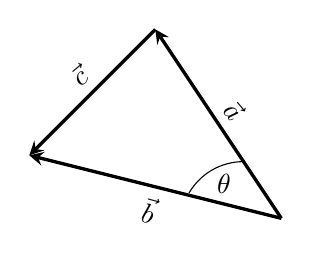
\begin{tikzpicture}[scale=.8]
		\draw[line width=1.2pt,stealth-](0,0)--(4,-1) node[rotate=-15,pos=0.5, below]{$\vec{b}$};
		\draw[line width=1.2pt,stealth-](2,2)--(4,-1) node[rotate=-50,pos=0.5, above]{$\vec{a}$};
		\draw[line width=1.2pt,-stealth](2,2)--(0,0) node[rotate=40,pos=0.5, above]{$\vec{c}$};
	        \draw(3.4,-.1) arc (90:150:1)node[pos=.3,below]{$\theta$};
	    \end{tikzpicture}
	\end{center}

	Sean $\vec{a},\vec{b},\vec{c}\in V_n$. Entonces demostraremos que
	$$\|\vec{c}\|^2=\|\vec{a}\|^2+\|\vec{b}\|^2-2\|\vec{a}\|\|\vec{b}\| \cos \theta$$
	Sea $\vec{a}+\vec{c}-\vec{b}=0$, entonces
	$$\|\vec{c}\|^2=\vec{c}\circ\vec{c}=(\vec{b}-\vec{a})\circ(\vec{b}-\vec{a})=\|\vec{b}\|^2-2\vec{a}\circ\vec{b}+\|\vec{a}\|^2$$
	Luego ya que $\vec{a}\circ \vec{b} = \|\vec{a}\|\|\vec{b}\|\cos \theta$, concluimos que,
	$$\|\vec{c}\|^2=\|\vec{a}\|^2+\|\vec{b}\|^2-2\|\vec{a}\|\|\vec{b}\| \cos \theta.$$\\


    %-------------------- 2.
    \item \textbf{\boldmath Si $\|\vec{a}\|=3$ y el ángulo entre $\vec{a}$ y $\vec{b}$ es $\dfrac{\pi}{2};$ ¿Cuál debe ser el valor de $\|\vec{b}\|$ para que $\vec{a}-\vec{b}$ sea perpendicular al vector $\vec{a}$ ?.\\\\
	Respuesta.-}\; Utilizando el teorema de senos se tiene que:
	\begin{center}
	    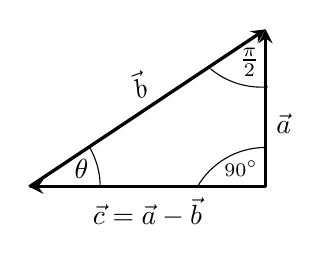
\begin{tikzpicture}[scale=1]
		\draw[line width=1.2pt,stealth-](0,0)--(3,0) node[rotate=0,pos=0.5, below]{$\vec{c}=\vec{a}-\vec{b}$};
		\draw[line width=1.2pt,-stealth](3,0)--(3,2) node[rotate=0,pos=0.4, right]{$\vec{a}$};
		\draw[line width=1.2pt,-stealth](0,0)--(3,2) node[rotate=20,pos=0.5, above]{$\vec{b}$};
		\draw(.9,0) arc (0:30:1)node[pos=.43,left]{$\theta$};
	        \draw(3,.5) arc (90:150:1)node[pos=.3,below]{\scriptsize$90^\circ$};
		\draw(2.3,1.5) arc (230:275:1)node[pos=.7,above]{$\frac{\pi}{2}$};
	    \end{tikzpicture}
	\end{center}
	$$\begin{array}{ccccc}
	    \dfrac{\sen \theta}{3}&=&\dfrac{\sen(90^\circ)}{\|\vec{b}\|}&=&\dfrac{\sen \frac{\pi}{2}}{\|\vec{c}\|}\\\\
	    \dfrac{\sen\theta}{3}&=&\dfrac{1}{\|\vec{b}\|}&=&\dfrac{1}{\|\vec{a}-\vec{b}\|}\\\\
	    \dfrac{\sen \theta}{\|\vec{a}-\vec{b}\|}&=&3&=&\|\vec{b}\|\\\\
	\end{array}$$
	Por lo tanto 
	$$\|\vec{b}|\|=3.$$

\end{enumerate}
